\documentclass[../main.tex]{subfiles}
\begin{document}
\setchapterstyle{kao}
\setchapterpreamble[u]{\margintoc}
\setchapterimage[6.5cm]{Images/intro.jpg}
\chapter[Introduction to the Standard Model]{Introduction to the Standard Model\footnotemark[0]}
\labch{IntroSM}
\section{Particles and Fundamental Interactions}
The Standard Model (SM) is the theory for all known fundamental interactions except gravity. How can we organize all the particles we observed so far? Is there an order? Obviously, the answer is yes. We can divide them between particles which mediate forces and particles which are affected by such forces but are not mediators or between elementary and non-elementary particles, stable and unstable and so on.\\
% \[
% \begin{aligned}
% &\text{Stable particle}&&\text{Reason}\\
% \hline
% &\gamma && \text{massless}\\
% &\text{lightest}\;\nu &&\text{lightest fermion}\\
% &e^- &&\text{lightest EM charged particle}\\
% &p &&\text{lightest baryon}\\
% \hline
% \end{aligned}
% \]
The \textbf{photon} $\gamma$ is massless so it cannot decay into anything. Nowadays we think that neutrinos have a small mass, so the \textbf{lightest neutrino} $\nu$ will be stable. \textbf{Electron} decay would violate U(1)$_{\text{EM}}$, it cannot decay into something that it is neutral so it has to be stable. The stability of the \textbf{proton} is due to the invariance of the Standard Model under baryon number transformations and the modern viewpoint is that this is an accidental symmetry of the Standard Model.\marginnote{We are not going to discuss accidental symmetries here.}\\
All the other particles instead can decay and we can learn something about them by looking at their lifetime because this tells us what kind of interactions they experience.
\begin{table}[h]
    \centering
    \begin{tabular}{lcc}
    \hline
    \rowcolor{gray!45}Decay & Lifetime $\tau$ & $c\tau$\\
    \hline
    \rowcolor{green!45}$n\to pe^-\overline{\nu}_e$ & 886\,s &$2.7\cdot10^8$\,km \\
    \rowcolor{green!45}$\mu^-\to e^-\nu_\mu\overline{\nu}_e$ & $2.2\cdot10^{-6}$\,s & 659\,m\\
    \rowcolor{green!45}$\pi^-\to \mu^-\nu\overline{\nu}_\mu$ & $2.6\cdot10^{-8}$\,s & 7.8\,m\\
    \rowcolor{green!45}$K_L\to\pi l\overline{\nu}_e$ & $5\cdot10^{-8}$\,s & 15\,m\\
    \rowcolor{green!45}$\tau\to l^-\overline{\nu}_e\nu_\tau$ & $0.3\cdot10^{-12}$\,s & 87\,$\mu$m\\
    \rowcolor{yellow!45}$\pi^0\to\gamma\gamma$ & $8.4\cdot10^{-12}$\,s & 25\,mm\\
    \hline\hline
    \rowcolor{gray!45}Resonance & Lifetime $\tau$ & $\Gamma/m$\\
    \hline
    \rowcolor{red!45}$\rho\to\pi\pi$ & $4.4\cdot10^{-24}$\,s & 0.2\\
    \rowcolor{red!45}$\Delta\to\pi\pi$ & $5.5\cdot10^{-24}$\,s & 0.1\\
    \hline
    \end{tabular}
    \caption{Colours indicate the different interactions: green for electroweak, yellow for electromagnetism and red for the strong force.}
    \label{tab:my_label}
\end{table}\\
% \renewcommand*{\arraystretch}{1.2}
% \begin{center}
%     \begin{tabular}{c}
%     $\kern-\nulldelimiterspace\left.
%     \begin{tabular}{@{}p{0.25\textwidth}p{0.25\textwidth}p{0.25\textwidth}@{}}
%     Decay & Lifetime $\tau$ & $c\tau$\\
%     \hline
%     $n\to pe^-\overline{\nu}_e$ & 886\,s &$2.7\cdot10^8$\,km \\
%     $\mu^-\to e^-\nu_\mu\overline{\nu}_e$ & $2.2\cdot10^{-6}$\,s & 659\,m\\
%     $\pi^-\to \mu^-\nu\overline{\nu}_\mu$ & $2.6\cdot10^{-8}$\,s & 7.8\,m\\
%     $K_L\to\pi l\overline{\nu}_e$ & $5\cdot10^{-8}$\,s & 15\,m\\
%     $\tau\to l^-\overline{\nu}_e\nu_\tau$ & $0.3\cdot10^{-12}$\,s & 87\,$\mu$m 
%   \end{tabular}\right\}$ {Electroweak interaction{\color{white}etic}}
% \\
%   $\kern-\nulldelimiterspace\left.
%   \begin{tabular}{@{}p{0.25\textwidth}p{0.25\textwidth}p{0.25\textwidth}@{}}
%   $\pi^0\to\gamma\gamma$ & $8.4\cdot10^{-12}$\,s & 25\,mm\\
%   \hline\hline
%   \end{tabular}\right\}$ Electromagnetic interaction
% \\
% $\kern-\nulldelimiterspace\left.
%   \begin{tabular}{@{}p{0.25\textwidth}p{0.25\textwidth}p{0.25\textwidth}@{}}
%   Resonance & Lifetime $\tau$ & $\Gamma/m$\\
%   \hline
%   $\rho\to\pi\pi$ & $4.4\cdot10^{-24}$\,s & 0.2\\
%   $\Delta\to\pi\pi$ & $5.5\cdot10^{-24}$\,s & 0.1\\
%   \end{tabular}\right\}$ {Strong interaction{\color{white}omagneti}}
% \end{tabular}
% \end{center}
Why are we interested in this list? Well, we see that some decays have a relatively long lifetime, typically of order of ($10^{-6}-10^{-8}$) s but as it is possible to see it can go up to some hundreds of seconds. This indicates us that they are mediated by \textbf{electroweak interaction}. The $\tau$ is also affected by electroweak interaction despite its shorter lifetime due to some suppressions in its three-body decay. Then there is a sort of gap, particles like $\pi^0$ have a smaller lifetime and they decay through \textbf{electromagnetic interaction}. Resonances are particles which decay so fast that can be only seen as exchange of energy. These decays are mediated by the \textbf{strong force}.\\
Just by looking at lifetimes we were able to identify the fundamental interactions described by the Standard Model:
\begin{itemize}
    \item \underline{Electromagnetism:} long range, $V(r)\sim\frac{1}{r}$
    \item \underline{Weak force:} ($\beta$ decay) short range, $V(r)\sim \frac{e^{-mr}}{r}$ for $m\sim100$\,GeV
    \item \underline{Strong force:} binds the nucleons to form the nuclei, short range because it is confined, $V(r)\sim r$ for $r\lesssim1$\,fm
\end{itemize}
Particles can be classified based on which force they experience. Moreover, we divide the particles in:
\begin{itemize}
    \item \underline{Leptons:} (weak and electromagnetic force) $e,\mu\tay,\nu_e,\nu_\mu,\nu_\tau$
    \item \underline{Hadrons:} (weak, electromagnetic and strong force) $\pi,p,n,k,\dots$
\end{itemize}
\section{Standard Model as an Effective Gauge Theory}
The Standard Model is based upon a gauge paradigm: the fundamental forces are mathematically described by gauge theories. How can we have all these manifestations described by a single representation? The Lagrangian is the same but in different phases: the \textbf{Coulomb phase} for the electromagnetic force, the \textbf{Higgs phase} for the weak force and the \textbf{confinement phase} for the strong force. What is the gauge group associated? 
\[
\text{G}=\text{SU}(3)_{\text{C}}\times\text{SU}(2)_{\text{EW}}\times\text{U}(1)_{\text{Y}}
\]
SU$(3)_{\text{C}}$ gives us 8 gluons, from SU$(2)_{\text{EW}}\times$U$(1)_{\text{Y}}$ we get $W_\mu^\pm, Z_\mu, \gamma$: these are the \textbf{gauge fields} of the SM, in this way we can explain these three forces. It is a renormalizable theory, symmetry breaking happens via a scalar field containing the Higgs boson. SM is an EFT, at high energies the coupling grows and there will be a Landau pole around $10^{24}$\,GeV.\\
The Standard Model is a theory of fields of spin 0, $\frac{1}{2}$ and 1, summarized in the table below.\marginnote{From \cite{SM}, Section 1.}
\begin{table}[h]
        \centering
        \begin{tabular}{c|c|c|c|c}
        \hline
        \rowcolor{gray!45}Field & SU$(3)_{\text{C}}$ & SU$(2)_{\text{EW}}$ & U$(1)_{\text{Y}}$ & SO(3,1) \\
        \hline
        \cellcolor{orange!45}$Q_L^i=\begin{pmatrix}
             u_L^i\\
             d_L^i 
        \end{pmatrix}$ & \cellcolor{orange!45}$\Box$ & \cellcolor{orange!45}$\Box$ & \cellcolor{orange!45}$+\frac{1}{6}$ &\cellcolor{orange!45} (2,1) \\
        \rowcolor{orange!45}$u_R^i$ & $\Box$ & 1 & $+\frac{2}{3}$ & (1,2) \\
        \rowcolor{orange!45}$d_R^i$ & $\Box$ & 1 & $-\frac{1}{3}$ & (1,2) \\
        \hline
        \cellcolor{orange!45}$L_L^i=\begin{pmatrix}\nu_L^i\\e_L^i\end{pmatrix}$ &\cellcolor{orange!45} 1 &\cellcolor{orange!45} $\Box$ &\cellcolor{orange!45} $-\frac{1}{2}$ &\cellcolor{orange!45} (2,1) \\
        \rowcolor{orange!45}$e_R^i$ & 1 & 1 & -1 & (1,2) \\
        \hline
        \rowcolor{blue!35}$G_\mu^{a=1,\dots,8}$ & Adj & 1 & 0 & (2,2)\\
        \rowcolor{blue!35}$W_\mu^{i=1,2,3}$ & 1 & Adj & 0 & (2,2)\\
        \rowcolor{blue!35}$B_\mu$ & 1 & 1 & 0 & (2,2)\\
        \hline
        \rowcolor{purple!45}$H$ & 1 & $\Box$ & $+\frac{1}{2}$ & (1,1)\\
        \hline
        \end{tabular}
        \caption{Field content in the Standard Model.}
        \labtab{SMfield}
    \end{table}\\
The \textbf{fermions} (matter fields), highlighted in orange in the table, are formed by quarks and leptons. Quarks come in triplet of colours, left-handed quarks and leptons come in doublets of weak isospin, where $i$ is the family index $i=1,2,3$. The fact that left- and right-handed fermions carry different weak isospin makes the Standard Model a chiral gauge theory. There is no right-handed neutrino because we do not need it now, we want the minimum number of fields which reproduce what is observed in nature, although there is evidence for neutrino masses from neutrino oscillations experiments. The threefold replication of quark-lepton families is one of the
puzzles whose explanation requires physics beyond the Standard Model.\\
The spin-1 particles are the \textbf{gauge bosons} associated with the fundamental interactions, highlighted in blue in the table: $G_\mu^a$ are the \textbf{gluons} of the \textbf{strong interaction}, $W_\mu^i$ and $B_\mu$ are the bosons of the \textbf{electroweak interaction}.\\
The last ingredient of the Standard Model is the \textbf{Higgs field}, the only spin-0 particle in the theory, highlighted in purple in the table. It is a complex scalar field and a doublet of weak isospin, coupling left- and right-handed fermions together.\\
In terms of these fields, the Lagrangian is:
\begin{kaobox}[frametitle=Standard Model Lagrangian]
\[
\pazocal{L}=\pazocal{L}_{\text{kin}}+\pazocal{L}_{\text{Yuk}}+\pazocal{L}_\theta-V(H)+\text{higher dimension operators}
\]
\end{kaobox}
where the four different pieces are:
\[
\left\{
\begin{aligned}
&\pazocal{L}_{\text{kin}}=-\frac{1}{4}(G_{\mu\nu}^a)^2-\frac{1}{4}(W_{\mu\nu}^i)^2-\frac{1}{4}(B_{\mu\nu})^2+|D_\mu H|^2+\sum_{\{\Psi\}}\sum_{j=1}^{3}\overline{\Psi}_ji\slashed{D}\Psi_j\\
&\pazocal{L}_\theta=\frac{\theta_0}{32\pi^2}G_{\mu\nu}^a\Tilde{G}^{\mu\nu,a}\\
&\pazocal{L}_{\text{Yuk}}=-\sum_{i,j=1}^3\left[\overline{Q}_L^i(Y_u)^{ij}H^cu_R^j+\overline{Q}_L^i(Y_d)^{ij}Hd_r^j+\overline{L}_L^i(Y_l)^{ij}He_R^j+\text{h.c}\right]\\
&V(H)=-\mu^2H^\dagger H+\lambda(H^\dagger H)^2
\end{aligned}
\right.
\]
$Y_u$, $Y_d$ and $Y_l$ are $3\times3$ matrices in flavour space. We know that $\Box$ of SU(2) is a pseudo-real representation, $H$ is the $\Box$ of SU(2) so it is always possible to form another $\Box$ of SU(2): $H^c:=i\sigma^2H^*$. It transforms as a doublet, we use it to build the Yukawa coupling and we use $H^c$ because it has hypercharge -1/2.\\
\subsection{Higgs Sector}
We now look at the potential $V(H)$. It must be invariant under SU(2), so there cannot be cubic terms.  First of all, we have to choose the right parametrization for the Higgs field $H$: there are 4 degrees of freedom, so we can put three of them on an exponential and the last one as a multiplicative constant.
\[
H(x)=e^{i\overset{\mathclap{\tikz \node {$\downarrow$} node [above=1ex] {\footnotesize  Nambu-Goldstone bosons};}}{\chi^i(x)}\sigma^i}\left(\begin{array}{c}0\\\frac{\phi(x)}{\sqrt{2}}\end{array}\right)
\]
Substituting this form of $H$ into the expression for the potential $V(H)$, we find out that this is only a function of $\phi(x)$:\marginnote{\hspace*{-1cm}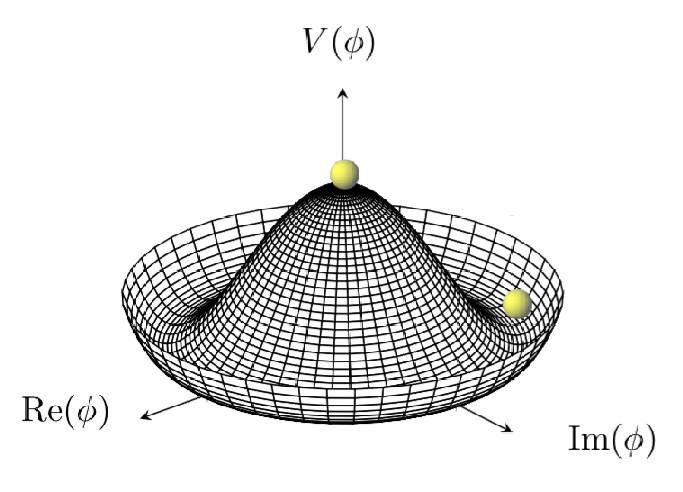
\includegraphics[width=0.7\textwidth]{Images/sombrero.png}\\
The Higgs potential has the shape of a Mexican hat ("\textit{sombrero potential}").}
\[
V(H)\xrightarrow[]{}V(\phi)=-\frac{1}{2}\mu^2\phi^2+\frac{1}{4}\lambda\phi^4
\]
% \begin{figure}[h!]
%     \centering
%     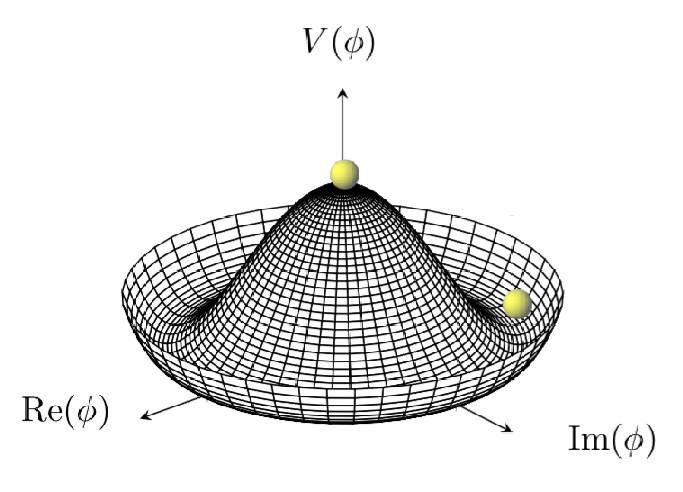
\includegraphics{Images/sombrero.png}
%     \caption{Higgs potential has the shape of a Mexican hat ("\textit{sombrero potential}").}
%     \labfig{sombrero}
% \end{figure}\\
This potential has two minima in $\pm v$, where $v=\sqrt{\frac{\mu^2}{\lambda}}=\langle\phi\rangle$: the field $\phi(x)$ can be written as its vacuum expectation value plus an excitation which turns out to be the Higgs boson:
\[
\phi(x)=\frac{v+h(x)}{\sqrt{2}}
\]
$h(x)$ is the radial excitation while $\chi(x)$ is the angular excitation: the latter costs no energy since $V(\phi)$ does not depend on $\chi$, therefore the NGBs are massless. \marginnote{From \cite{schwartz}, Section 29.1.}We have the SSB mechanism here: how do we understand which symmetry we are breaking? We write the vev and see what symmetry is left invariant.
\[
\langle H(x)\rangle=\frac{1}{\sqrt{2}}\begin{pmatrix}
    0\\v
\end{pmatrix}
\]
Now we act with a combination of generators from SU(2)$\times$U(1), which is $a_i\frac{\sigma_i}{2}+a_0Y$. We want to see when $(a_i\frac{\sigma_i}{2}+a_0Y)\langle H(x)\rangle=0$.
\begin{align*}
\left(a_i\frac{\sigma_i}{2}+a_0Y\right)\langle H(x)\rangle&=\frac{1}{2}\left(\begin{array}{cc}
    2a_0+a_3 & a_1-ia_2 \\
    a_1+ia_2 & 2a_0-a_3
\end{array}\right)\begin{pmatrix}
    0\\1
\end{pmatrix}\\
&=\frac{1}{2}\begin{pmatrix}
    a_1-ia_2\\2a_0-a_3
\end{pmatrix}
\begin{pmatrix}
    0\\1
\end{pmatrix}=\begin{pmatrix}
    0\\0
\end{pmatrix}\Rightarrow\left\{\begin{aligned}
    &a_1=a_2=0\\
    &a_0=\frac{1}{2}a_3
\end{aligned}\right.
\end{align*}
The \textbf{unbroken generator} is $Q=T_3+\frac{1}{2}Y$, the Higgs scalar potential breaks SU$(2)_{\text{EW}}\times$U$(1)_{\text{Y}}$ into U$(1)_{\text{Q}}$, i.e. 3+1 generators are broken into 1, resulting in 3 massless modes.\\
We now want to see masses and couplings, so we move in the unitary gauge where $\chi^i=0$. In the unitary gauge the potential will depend on $h(x)$, resulting in:
\[
V(H)=\frac{1}{2}m_h^2h^2(x)+\lambda vh^3(x)+\frac{1}{4}\lambda h^4(x)+\text{constant terms}
\]
with $m_h^2=2\mu^2=2v^2\lambda$. We need the masses for the vector bosons, so we look at the kinetic term
$|D_\mu H|^2=(D_\mu H)^\dagger(D_\mu H)$. Here the covariant derivative is defined as:
\[
D_\mu H=\frac{1}{\sqrt{2}}\left[\partial_\mu-\frac{i}{2}(gW_\mu^i\sigma^i+g'Y_WB_\mu)\right]\begin{pmatrix}0 \\ v+h(x)\end{pmatrix}
\]
where $g$ is the gauge coupling of SU(2) and $g'$ the gauge coupling of U(1)$_{\text{Y}}$.\\
Before proceeding with the calculations, we define $W_\mu^\pm:=\frac{1}{\sqrt{2}}(W_\mu^1\mp iW_\mu^2)$ and $\sigma^\pm:=\frac{1}{2}(\sigma^1\pm i\sigma^2)$, so that it is possible to write:
\begin{align*}
(W_\mu^+\sigma^++W_\mu^-\sigma^-)=&\frac{1}{2\sqrt{2}}(W_\mu^1-iW_\mu^2)(\sigma^1+i\sigma^2)+\frac{1}{2\sqrt{2}}(W_\mu^1+iW_\mu^2)(\sigma^1-i\sigma^2)\\
=&\frac{1}{2\sqrt{2}}(W_\mu^1\sigma^1+\cancel{iW_\mu^1\sigma^2}-\cancel{iW_\mu^2\sigma^1}+W_\mu^2\sigma^2)\\
&+\frac{1}{2\sqrt{2}}(W_\mu^1\sigma^1-\cancel{iW_\mu^2\sigma^2}+\cancel{iW_\mu^2\sigma^1}+W_\mu^2\sigma^2)\\
=&\frac{1}{\sqrt{2}}(W_\mu^1\sigma^1+W_\mu^2\sigma^2)
\end{align*}
From which it follows that:
\[
W_\mu^1\sigma^1+W_\mu^2\sigma^2+W_\mu^3\sigma^3=\sqrt{2}(W_\mu^+\sigma^++W_\mu^-\sigma^-)+W_\mu^3\sigma^3
\]
$D_\mu H$ now becomes:
\[
D_\mu H=\frac{1}{\sqrt{2}}\begin{pmatrix}0 \\ \partial_\mu h(x)\end{pmatrix}-\frac{i}{2\sqrt{2}}(gW_\mu^3\sigma^3+g'Y_WB_\mu)\begin{pmatrix}0 \\ v+h(x)\end{pmatrix}-\frac{ig}{2}(W_\mu^+\sigma^++W_\mu^-\sigma^-)\begin{pmatrix}0 \\ v+h(x)\end{pmatrix}
\]
When we act with $\sigma^3$, $\sigma^+$ and $\sigma^-$ on $H(x)$ we get:
\[
\left\{
\begin{aligned}
&\sigma^3H(x)=\left(\begin{array}{cc}
    1 & 0 \\
    0 & -1
\end{array}\right)\left(\begin{array}{c}
  0 \\
  v+h(x)
\end{array}\right)=-\left(\begin{array}{c}
  0 \\
  v+h(x)
\end{array}\right) \\
&\sigma^+H(x)=\left(\begin{array}{cc}
    0 & 1 \\
    0 & 0
\end{array}\right)\left(\begin{array}{c}
  0 \\
  v+h(x)
\end{array}\right)=+\left(\begin{array}{c}
  v+h(x) \\
  0
\end{array}\right) \\
&\sigma^-H(x)=\left(\begin{array}{cc}
    0 & 0 \\
    1 & 0
\end{array}\right)\left(\begin{array}{c}
  0 \\
  v+h(x)
\end{array}\right)=\left(\begin{array}{c}
  0 \\
  0
\end{array}\right)
\end{aligned}
\right.
\]
Substituting this into the previous expression for $D_\mu H$, one finds:
\[
D_\mu H=\frac{1}{\sqrt{2}}\begin{pmatrix}0 \\ \partial_\mu h(x)\end{pmatrix}+\frac{i}{2\sqrt{2}}(gW_\mu^3-g'Y_WB_\mu)\begin{pmatrix}0 \\ v+h(x)\end{pmatrix}-\frac{ig}{2}W_\mu^+\begin{pmatrix}v+h(x) \\ 0 \end{pmatrix}
\]
With the same strategy, we compute $(D_\mu H)^\dagger$:
\begin{align*}
(D_\mu H)^\dagger=&\begin{pmatrix}0 & v+h(x)\end{pmatrix}\frac{1}{\sqrt{2}}\left[\partial_\mu+\frac{i}{2}(g\sigma^iW_\mu^i+g'Y_WB_\mu)\right]\\
=&\frac{1}{\sqrt{2}}\begin{pmatrix}0 & \partial_\mu h(x)\end{pmatrix}+\frac{i}{2\sqrt{2}}\begin{pmatrix}0 & v+h(x)\end{pmatrix}(g\sigma^3W_\mu^3+g'Y_WB_\mu)\\
&+\frac{ig}{2}\begin{pmatrix}0 & v+h(x)\end{pmatrix}(\sigma^+W_\mu^++\sigma^-W_\mu^-)\marginnote{We act with the $\sigma$ matrices on the row vector: $\sigma^3$ changes its sign as before, $\sigma^+$ gives a zero while $\sigma^-$ flips it.}\\
=&\frac{1}{\sqrt{2}}\begin{pmatrix}0 & \partial_\mu h(x)\end{pmatrix}-\frac{i}{2\sqrt{2}}\begin{pmatrix}0 & v+h(x)\end{pmatrix}(gW_\mu^3-g'Y_WB_\mu)\\
&+\frac{ig}{2}\begin{pmatrix}v+h(x) & 0\end{pmatrix}W_\mu^-
\end{align*}
We can finally write the full form of $|D_\mu H|^2$:
\begin{align*}
|D_\mu H|^2&=(D_\mu H)^\dagger(D_\mu H)\\
&=\frac{1}{2}(\partial_\mu h(x))^2+\frac{(v+h(x))^2}{8}(gW_\mu^3-g'B_\mu)^2+\frac{g^2}{4}(v+h(x))^2W_\mu^+W_\mu^-\\
&=\frac{1}{2}(\partial_\mu h(x))^2+\frac{v^2}{8}(gW_\mu^3-g'B_\mu)^2\left(1+\frac{h(x)}{v}\right)^2+\frac{g^2v^2}{4}W_\mu^+W_\mu^-\left(1+\frac{h(x)}{v}\right)^2
\end{align*}
At this point, we can identify the mass of the $W$ boson as:
\begin{kaobox}[frametitle=Mass of the $W$ boson]
\[
m_W:=\frac{1}{2}gv
\]    
\end{kaobox}
To explicitly see the mass of the $Z$ boson $m_Z$ we perform a rotation. Let $A_\mu$ be the massless field and $Z_\mu$ the massive one:
\[
\left(\begin{array}{c}
     A_\mu \\
     Z_\mu
\end{array}\right)=\left(\begin{array}{cc}
    \cos\theta_w & \sin\theta_w \\
    -\sin\theta_w & \cos\theta_w
\end{array}\right)\left(\begin{array}{c}
     B_\mu \\
     W_\mu^3 
\end{array}\right)
\]
From this rotation, it follows that:
\begin{equation}
\labeq{azbasis}
\left\{
\begin{aligned}
&A_\mu=\sin\theta_wW_\mu^3+\cos\theta_wB_\mu\\
&Z_\mu=\cos\theta_wW_\mu^3-\sin\theta_wB_\mu
\end{aligned}
\right.
\Leftrightarrow
\left\{
\begin{aligned}
&B_\mu=\cos\theta_wA_\mu-\sin\theta_wZ_\mu\\
&W_\mu^3=\sin\theta_wA_\mu+\cos\theta_wZ_\mu
\end{aligned}
\right.
\end{equation}
$\theta_w$ is the \href{https://en.wikipedia.org/wiki/Steven_Weinberg}{Weinberg} angle. To write the mass term $m_Z^2$ in the expression of $|D_\mu H|^2$, we have to perform some tricks:
\[
{\color{red}\frac{g^2+g'^2}{g^2+g'^2}}\frac{v^2}{8}(gW_\mu^3-g'B_\mu)^2=\frac{m_Z^2}{2}\left(\frac{g}{\sqrt{g^2+g'^2}}W_\mu^3-\frac{g'}{\sqrt{g^2+g'^2}}B_\mu\right)^2
\]
To obtain the desired result, we express $\theta_w$ in terms of the couplings $g$ and $g'$:
\begin{equation}
\labeq{thetaw}  
\sin\theta_w:=\frac{g'}{\sqrt{g^2+g'^2}} \quad \cos\theta_w:=\frac{g}{\sqrt{g^2+g'^2}} \quad \tan\theta_w=\frac{g'}{g}
\end{equation}
In this way, it is possible to define:
\begin{kaobox}[frametitle=Mass of the $Z$ boson]
\[
m_Z:=\frac{1}{2}v\sqrt{g^2+g'^2}=\frac{1}{2}\frac{gv}{\cos\theta_w}=\frac{m_W}{\cos\theta_w}\marginnote{The subscript with capital W is for the $W$ boson, while the one with small w is for the Weinberg angle.}
\]    
\end{kaobox}
$|D_\mu H|^2$ now can be written as:
\[
|D_\mu H|^2=\frac{1}{2}(\partial_\mu h(x))^2+\frac{1}{2}m_Z^2Z_\mu Z^\mu\left(1+\frac{h(x)}{v}\right)^2+m_W^2W_\mu^+W_\mu^-\left(1+\frac{h(x)}{v}\right)^2
\]
We have the three fields that will acquire mass, the only remaining massless field is the photon. 
\subsection{Fermion Sector}\marginnote{From \cite{schwartz}, Section 29.3.}
Lastly, we want to understand how to couple the electroweak gauge bosons to fermions. It turns out that the theory of weak interactions is chiral and maximally parity-violating: the SU(2) gauge bosons \textit{only} couple to \textbf{left-handed} fermions.\marginnote{This fact was originally deduced by observations at low energy, well before the $W$ and $Z$ bosons were produced in colliders.} Unfortunately, there is no compelling explanation of \textit{why} the weak interaction must couple this way.\\
The left-handed leptons $(e,\nu_e,\mu,\nu_\nu,\tau,\nu_\tau)$ and quarks $(u,d,c,s,t,b,)$ pair up to transform under SU(2) in the fundamental representation. The three \textbf{generations} of SU(2) doublet of quarks and leptons are:
\[
L_L^i=\begin{pmatrix}
    \nu_{eL}\\
    e_L
\end{pmatrix}, \begin{pmatrix}
    \nu_{\mu L}\\
    \mu_L
\end{pmatrix}, \begin{pmatrix}
    \nu_{\tau L}\\
    \tau_L
\end{pmatrix}
\quad
Q_L^i=\begin{pmatrix}
    u_L\\
    d_L
\end{pmatrix}, \begin{pmatrix}
    c_L\\
    s_L
\end{pmatrix}, \begin{pmatrix}
    t_L\\
    b_L
\end{pmatrix}
\]
$i=1,2,3$ is the index of the generation. These all transform as left-handed Weyl spinors, i.e. in the $\left(\frac{1}{2},0\right)$ representation of the Lorentz group [\refsec{replor}]. The right-handed fermions happen to be SU(2) singlet so they are uncharged under weak interaction.
\[
e_R^i=\{e_R,\mu_R,\tau_R\} \quad u_R^i=\{u_R,c_R,t_R\} \quad d_R^i=\{d_R,s_R,b_R\}
\]
They all transform as right-handed Weyl spinors under the Lorentz group.\marginnote{Again, right-handed neutrinos are not included despite observations suggest their existence.}\\
Consider now the electroweak kinetic term in $Q_L^i$:
\[
\overline{Q}_L^ii\slashed{D}Q_L^i=\overline{Q}_L^ii\gamma^\mu\left[\partial_\mu-\frac{i}{2}(gW_\mu^i\sigma^i-g'YB_\mu)\right]Q_L^i
\]
We use the same substitution as before with $W_\mu^+$ and $W_\mu^-$ to write:
\[
\overline{Q}_L^ii\slashed{\partial}Q_L^i+\overline{Q}_L^i\gamma^\mu\left[\frac{g}{\sqrt{2}}(W_\mu^+\sigma^++W_\mu^-\sigma^-)+\left(gW_\mu^3T_3+g'B_\mu \frac{1}{2}Y\right)\right]Q_L^i
\]
Now we change to the $A_\mu-Z_\mu$ basis by using \refeq{azbasis} which gives us:
\begin{align*}
gW_\mu^3T_3+g'B_\mu\frac{1}{2}Y&=gT_3(\sin\theta_wA_\mu+\cos\theta_wZ_\mu)+\frac{1}{2}g'Y(\cos\theta_wA_\mu-\sin\theta_wZ_\mu)\\
&=A_\mu\left(gT_3\sin\theta_w+\frac{1}{2}g'Y\cos\theta_w\right)+Z_\mu\left(gT_3\cos\theta_w-\frac{1}{2}g'Y\sin\theta_w\right)
\end{align*}
But we know from \refeq{thetaw} how to express $\sin\theta_w$ and $\cos\theta_w$ in terms of the couplings $g$ and $g'$:
\[
gT_3{\color{green}\sin\theta_w}+\frac{1}{2}g'Y{\color{blue}\cos\theta_w}=T_3{\color{green}\frac{{\color{black}g}g'}{\sqrt{g^2+g'^2}}}+\frac{1}{2}Y{\color{blue}\frac{g{\color{black}g'}}{\sqrt{g^2+g'^2}}}=\frac{gg'}{\sqrt{g^2+g'^2}}\left(T_3+\frac{1}{2}Y\right):=e\cdot Q
\]
where in the last step we have defined:
\[
e:=\frac{gg'}{\sqrt{g^2+g'^2}}\xleftrightarrow[]{}\frac{1}{e^2}=\frac{1}{g^2}+\frac{1}{g'^2} \quad Q:=T_3+\frac{1}{2}Y
\]
This was for the term proportional to $A_\mu$, now we use this result to compute the term proportional to $Z_\mu$:
\begin{align*}
gT_3{\color{blue}\cos\theta_w}-g'{\color{red}\frac{1}{2}Y}{\color{green}\sin\theta_w}&={\color{blue}\frac{g{\color{black}g}}{\sqrt{g^2+g'^2}}}T_3-{\color{red}(Q-T_3)}{\color{green}\frac{g'{\color{black}g'}}{\sqrt{g^2+g'^2}}}\\
&=\sqrt{g^2+g'^2}T_3-Q\frac{g'^2}{\sqrt{g^2+g'^2}}\frac{\sqrt{g^2+g'^2}}{\sqrt{g^2+g'^2}}\\
&=\sqrt{g^2+g'^2}T_3-\sqrt{g^2+g'^2}Q\frac{g'^2}{g^2+g'^2}\\
&=\frac{g}{\cos\theta_w}(T_3-\sin^2\theta_wQ)
\end{align*}
In the last step we used from \refeq{thetaw} that $\sqrt{g^2+g'^2}=\frac{g}{\cos\theta_w}$ and $\sin^2\theta_w=\frac{g'^2}{g^2+g'^2}$.\\
At the end of the day, putting everything together we have:
\begin{align*}
\overline{Q}_L^ii\slashed{D}Q_L^i=&\underbrace{\overline{Q}_L^ii\gamma^\mu(\partial_\mu-ieQA_\mu)Q_L}_{\text{photons interaction}}\\
&+\underbrace{\frac{g}{\sqrt{2}}\overline{Q}_L^i\gamma^\mu(\sigma^+W_\mu^++\sigma^-W_\mu^-)Q_L^i}_{\text{$W$ interaction}}\\
&+\underbrace{\frac{g}{\cos\theta_w}\gamma^\mu Z_\mu\overline{Q}_L^i(T_3-\sin^2\theta_wQ)Q_L^i}_{\text{$Z$ interaction}}
\end{align*}
For $Q_L^i$ [\reftab{SMfield}], $Q$ is given by the matrix:
\[
Q=\mqty(\dmat{+\frac{2}{3},-\frac{1}{3}})
\]
while for $u_R$ and $d_R$ we have only one number since $T_3=0$. If we put everything together we get:
\begin{equation}
\labeq{Yuk}
\begin{aligned}
\overline{Q}_L^ii\slashed{D}Q_L^i=&\overline{u}_L^ii\gamma^\mu\left[\partial_\mu-\frac{2}{3}ieA_\mu\right]u_L^i+\overline{d}_L^ii\gamma^\mu\left[\partial_\mu+\frac{1}{3}ieA_\mu\right]d_L^i\\
&+\frac{g}{\sqrt{2}}\overline{u}_L^i\gamma^\mu W_\mu^+d_L^i+\frac{g}{\sqrt{2}}\overline{d}_L^i\gamma^\mu W_\mu^-u_L^i\\
&+\frac{g}{\cos\theta_w}Z_\mu\left[\overline{u}_L^i\gamma^\mu\left(\frac{1}{2}-\frac{2}{3}\sin^2\theta_w\right)u_L^i\right]\\
&+\frac{g}{\cos\theta_w}Z_\mu\left[\overline{d}_L^i\gamma^\mu\left(-\frac{1}{2}+\frac{1}{3}\sin^2\theta_w\right)d_L^i\right]
\end{aligned}
\end{equation}
The last thing left to do is to discuss fermion masses.\marginnote{From \cite{schwartz}, Section 29.3.2.} In fact, at this point we do not really have a left- and a right-handed electron but rather two separate unrelated fields which happen to have the same electric charge. In QED, left- and right-handed fermions were connected by a Dirac mass term. However, a mass term like $\overline{e}_Le_R$ explicitly breaks SU(2) invariance and therefore is forbidden.\\
Focus now just on quarks, we look at the Yukawa Lagrangian in the unitary gauge.
\begin{align*}
\pazocal{L}_{\text{Yuk}}&\supset-\overline{Q}_L^iY_u^{ij}\frac{1}{\sqrt{2}}\begin{pmatrix}
    1\\0
\end{pmatrix}(v+h)u_R^j-\overline{Q}_L^iY_d^{ij}\frac{1}{\sqrt{2}}\begin{pmatrix}
    0\\1
\end{pmatrix}(v+h)d_R^j+\text{h.c}\\
&=-\frac{vY_u^{ij}}{\sqrt{2}}\left(1+\frac{h}{v}\right)\overline{u}_L^iu_R^j-\frac{vY_d^{ij}}{\sqrt{2}}\left(1+\frac{h}{v}\right)\overline{d}_L^id_R^j+\text{h.c}
\end{align*}
We can see that there are two $3\times3$ Yukawa matrices, which contain a lot of parameters for just a few masses. If it were not for gauge interactions, we could just diagonalize these matrices and the masses would be the only physical parameters. The term $\frac{1}{\sqrt{2}}vY_u^{ij}$ represents a mass term but the Yukawa matrix is not diagonal: we have to perform two unitary transformations in order to diagonalize it.
\[
\left\{
\begin{aligned}
&u_L^i=(U_L)_{ij}u_L^j\\
&u_R^i=(U_R)_{ij}u_R^j
\end{aligned}
\right.
\quad 
U_L,U_R\in\text{SU}(3):
\left\{
\begin{aligned}
&Y_u\to U_L^\dagger Y_uU_R:=Y_u^{\text{diag}}\\
&Y_u^\dagger\to U_R^\dagger Y_u^\dagger U_L
\end{aligned}
\right.
\]
The same process can be repeated for $Y_d$. Now we have these diagonal matrices with, in general, complex entries. We want real masses, so we perform a phase transformation.
\[
u_R^i\to e^{i\phi_i}u_R^i\Rightarrow Y_u^{\text{diag}}=\mqty(\dmat{y_u,y_c,y_t})
\]
The Yukawa Lagrangian now gets written as:
\[
\pazocal{L}_{\text{Yuk}}=-\overline{u}^i_L\mqty(\dmat{m_u,m_c,m_t})_{ij}u^j_R\left(1+\frac{h}{v}\right)+\text{h.c.}-\overline{d}^i_L\mqty(\dmat{m_d,m_s,m_b})_{ij}d^j_R\left(1+\frac{h}{v}\right)+\text{h.c.}
\]
This gives us the masses of the quarks, where we have defined $m_i$ as $m_i:=\frac{1}{\sqrt{2}}vY_{ii}$. There is also interaction with $h(x)$, but the flavour does not change in the interaction with the Higgs boson.\\
What happens to the kinetic term after this rotation? If we look at \refeq{Yuk}, we notice that for $u_L$ and $d_L$ we have the term $\overline{u}_L\gamma^\mu W_\mu^+d_L$ which mixes the two fields. After the rotation, this becomes:
\[
\frac{g}{\sqrt{2}}\overline{u}_L^i\gamma^\mu W_\mu^+d_L^i\to\frac{g}{\sqrt{2}}\overline{u}_L^i\gamma^\mu(U_L^\dagger D_L)_{ij}W_\mu^+d_L^j=\frac{g}{\sqrt{2}}\overline{u}_L^i\gamma^\mu(V_{\text{CKM}})_{ij}W_\mu^+d_L^j
\]
where $V_{\text{CKM}}:=U_L^\dagger D_L$. Hence, all of the interesting mixing effects are given by a single matrix known as the \href{https://en.wikipedia.org/wiki/Nicola_Cabibbo}{Cabibbo}-\href{https://en.wikipedia.org/wiki/Makoto_Kobayashi_(physicist)}{Kobayashi}-\href{https://en.wikipedia.org/wiki/Toshihide_Maskawa}{Maskawa} (CKM) matrix.\marginnote{This topic is discussed more in detail in the course \textit{Weak Interactions in the Standard Model and Beyond}, by prof. Contino (again) and Nardecchia but I wanted to include it here for completeness and to have a nice ending to the chapter.} The CKM matrix is a complex unitary $3\times3$ matrix, therefore it has nine real degrees of freedom. If it was real, it would be an O(3) matrix, with three degrees of freedom corresponding to three rotation angles. Being it complex, there are three angles and six phases in $V_{\text{CKM}}$. However, we can use the U(1)$^6$ symmetry under which the masses are invariant to set some phases to zero. If all the U(1) rotations are the same, then $V_{\text{CKM}}$ is unchanged and it is possible to eliminate only five phases, remaining with four degrees of freedom: three mixing angles $\theta_{12}$, $\theta_{13}$, $\theta_{23}$ and one phase $\delta$. The angle $\theta_{12}$ is known as the \textbf{Cabibbo angle}, it is the rotation angle between the first two generations and the only parameter relevant to hadronic physics involving light quarks $(u,d,s)$, so it was very important historically.\\
If we had only two generations, we would have a $2\times2$ complex matrix with four real degrees of freedom: one rotation angle and three phases. with the U(1)$^4$ symmetry it is possible to remove three phases, so in the end there is only one parameter, the Cabibbo angle. In particular, the CKM matrix can be taken as \textbf{real}. If this is the case, then there can be no CP violation. Historically, CP violation was observed in the kaon system well before the third generation was discovered and a third generation was predicted as necessary for CP violation. 
% From here there is flavour violation in the SM. This SU(3) matrix has 8 parameters, 3 angles and 5 phases with only one phase being a physical one. Lastly, we can perform another transformation in \refeq{Yuk2}:
% \[
% \left\{
% \begin{aligned}
% &u_i\to e^{i\theta_i}u_i\\
% &d_i\to e^{i\Tilde{\theta}_i}d_i
% \end{aligned}
% \right.
% \]
% If all the transformations for up were equal to the transformations for down, we would not have to do them because there will be an overall global phase factor. The only phase responsible for CP violation in the SM is the one corresponding to $\theta_i=-\Tilde{\theta}_i=\theta$.
\end{document}